\documentclass[conference]{IEEEtran}
\IEEEoverridecommandlockouts
% The preceding line is only needed to identify funding in the first footnote. If that is unneeded, please comment it out.
\usepackage{cite}
\usepackage{amsmath,amssymb,amsfonts}
\usepackage{algorithmic}
\usepackage{graphicx}
\usepackage{textcomp}
\usepackage{xcolor}
\def\BibTeX{{\rm B\kern-.05em{\sc i\kern-.025em b}\kern-.08em
    T\kern-.1667em\lower.7ex\hbox{E}\kern-.125emX}}
\begin{document}

\title{The Observatory}

\author{\IEEEauthorblockN{1\textsuperscript{st} Fabio Plunser}
\and
\IEEEauthorblockN{2\textsuperscript{nd} Dominik Barbist}
\and
\IEEEauthorblockN{3\textsuperscript{rd} Florian Gruber}
}

\maketitle

\section{Introduction}
For this project, we need to implement a system that can detect unknown faces in a given environment (IoT device/cameras). 
For that, it will use a camera to collect images, process them on the edge device, and send the processed images to the cloud. 
In the cloud, we will use Amazon Rekognition to analyze the faces and compare them with a database (S3) of known faces. 
If an unknown face is detected, we will send a signal to the edge device to trigger an alarm for the responding IoT device.
There are a couple of hurdles we need to overcome for this project. A high level of parallelism is needed to process the 
images sent from at least 5 video sources.
\\
\textbf{Main Steps:}
\begin{itemize}
    \item \textbf{Data Collection:} We need to collect images from the sensors and send them over the edge device to the cloud.
    \item \textbf{Data Processing:} We need to do preprocessing on the images to extract the relevant information (faces) on the edge device.
    \item \textbf{Data Storage:} We need to store the processed images in the cloud (S3).
    \item \textbf{Data Analysis:} We need to analyze the faces in the cloud and cross-reference them with faces in the database.
    \item \textbf{Signal Processing:} We need to send a signal to the edge device to notify the IoT device about an unknown face and subsequently trigger an alarm.
    \item \textbf{User Interface:} We need to provide a user interface for the user to view the unknown faces (maybe) and disarm the alarm.
\end{itemize}

\section{System architecture}
\begin{itemize}
    \item \textbf{Data Collection:} At the start, we will emulate the data collection by using WiseNet. Later, we will use a real camera to collect data (maybe).
    \item \textbf{Data Processing:} For the data preprocessing, we will use OpenCV, and for the face recognition, we will use YOLO(not sure about the exact version).
    \item \textbf{Data Storage:} We will use AWS S3 to store the processed images.To save bandwidth, we will only store(required for Amazon Rekognition) the processed images (faces) 
                                    and not the raw images. To keep track of the processed images, we will use a database to link an IoT device with their processed images.
    \item \textbf{Data Analysis:} After the images are stored in S3, the edge device will send a signal to a Lambda function which will trigger the face recognition 
                                    process in Amazon Rekognition.
    \item \textbf{Signal Processing:} If an unknown face is detected, the Lambda function will send a signal to the edge device to trigger an alarm for a given IoT device.
    \item \textbf{User Interface:} We will use a simple web interface to display the unknown faces and disarm the alarm.
\end{itemize}
% Describe your system in detail, including a figure for your architectural diagram (IoT, Edge, Cloud layers, components developed and services used).

\begin{figure}[h!]
    \centering
    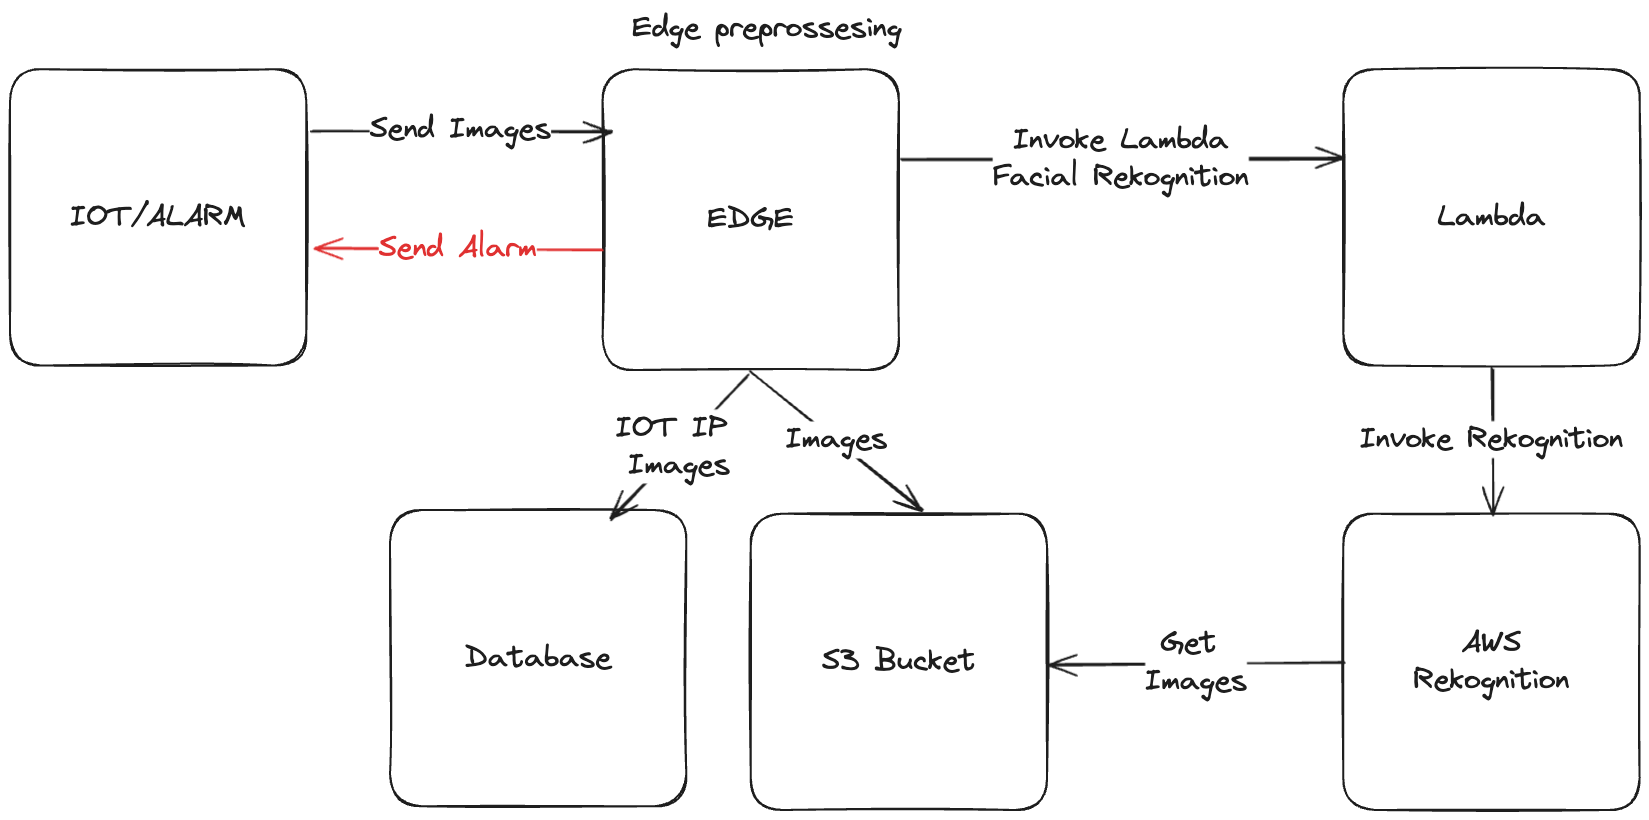
\includegraphics[width=1\linewidth]{images/architecture.excalidraw.png}
    \caption{Example of your architectural diagram.}
    \label{fig:enter-label}
\end{figure}

\section{Implementation details}
\subsection{Data Collection}
\begin{itemize}
    \item \textbf{WiseNet:} ...
    \item \textbf{Camera:} ...
\end{itemize}
\subsection{Data Processing}
\begin{itemize}
    \item \textbf{OpenCV:} ...
    \item \textbf{YOLO:} ...
\end{itemize}
\subsection{Data Storage}
\begin{itemize}
    \item \textbf{AWS S3:} ...
    \item \textbf{Database:} ...
\end{itemize}
\subsection{Data Analysis}
\begin{itemize}
    \item \textbf{Amazon Rekognition:} ...
\end{itemize}
\subsection{Signal Processing}  
\begin{itemize}
    \item \textbf{Lambda Function:} ...
    \item \textbf{NATS:} ...
\end{itemize}
\subsection{User Interface}
\begin{itemize}
    \item \textbf{Web Interface:} ...
    \item \textbf{Disarm Alarm:} ...
\end{itemize}

\section{Evaluation}
% Evaluation of the response time and scalability (number of devices and traffic) to prove the correctness of your implementation. 
% The more detailed the better. 

\end{document}
